\chapter{Experiments and Results}
\label{chap:results}

This chapter reports the empirical evaluation of the conformal uncertainty quantification framework developed in Chapter~\ref{chap:methodology} and implemented in Chapter~\ref{chap:implementation}. The evaluation is organised around the six research objectives set out in Section~\ref{sec:objectives}: whether the framework achieves the nominal coverage level on held-out market data, how the rolling window behaves as recent surfaces enter and leave the calibration set, whether Mondrian binning addresses spatially uneven coverage, whether the projection reliably eliminates violations of the calendar and discrete butterfly conditions, and whether the resulting bands are sharp enough to be practically informative. Section~\ref{sec:exp_setup} specifies the dataset and evaluation protocol. Section~\ref{sec:exp_calibration} examines quantile behaviour during the calibration phase. Section~\ref{sec:exp_arbitrage} presents the projection results for both scores and establishes why Score B is the recommended construction. Section~\ref{sec:exp_ablation} reports the full Score A versus Score B comparison across coverage, sharpness, and projection tractability. Sections~\ref{sec:exp_coverage} and~\ref{sec:exp_sharpness} then report the detailed coverage and sharpness results for Score B as the primary framework. Section~\ref{sec:exp_summary} summarises the findings.

\section{Experimental Setup}
\label{sec:exp_setup}

The raw dataset comprises 56 S\&P 500 (SPX) option surface files with collection dates between 11 December 2025 and 15 August 2026. The option chains were obtained through OpenBB using its Cboe provider and stored in a WRDS-compatible CSV schema, as described in Section~\ref{sec:impl_data}. They are loaded by the \texttt{WRDSOptionsDataset} class, whose name refers to the expected schema rather than the source of the observations. Ten files carry collection dates on which no regular Cboe trading session occurred and are therefore excluded before the analysis dataset is constructed. The early-close session on 24 December 2025 is retained. This calendar filter leaves 46 surfaces spanning 11 December 2025 to 11 August 2026.

The first 15 retained surfaces, dated from 11 December 2025 to 17 February 2026, form the initial calibration period. The remaining 31 surfaces, dated from 3 March 2026 to 11 August 2026, are evaluated sequentially using a walk-forward procedure. At each evaluation step, the band is constructed from the preceding calibration window before the current surface is added, thereby preventing future observations from entering the calibration data. Missing dates are neither filled nor interpolated. Consequently, a rolling window of size $L=5$ contains the five most recent available surfaces rather than five consecutive calendar days.

Within every retained surface, a fixed coordinate-stratified mask assigns 80\% of the available quotes to the GNO context set and holds out 20\% as target observations. The same deterministic masking rule, with seed 2026, is used for both score constructions. Coverage, prediction error, and band width are evaluated only at these held-out target locations. Each retained surface contains between 8{,}677 and 11{,}325 quotes in the transformed coordinate domain $D=(0.01,1)\times(-1.5,0.5)$, corresponding to 6{,}943--9{,}058 context points and 1{,}734--2{,}267 held-out target points per surface.

The structure of the filtered dataset is illustrated in Figure~\ref{fig:dataset_overview} of Chapter~\ref{chap:implementation}, which shows the option quote count and the calibration/evaluation timeline across the 46 retained surfaces.

The point predictor underlying the framework is the pre-trained GNO of Gonon, Jacquier, and Wiedemann~\cite{gonon2024operator}, loaded from the checkpoint \texttt{train/store/9448705/checkpoints/checkpoint\_final.pt}. The model has 102,529 parameters and is run in inference mode without retraining or fine-tuning on the SPX data used here. The conformal layer is applied post-hoc, as described in Chapter~\ref{chap:methodology}: the GNO point predictions are fixed, and calibration and band construction are performed solely through the conformal pipeline. The configuration is fixed before walk-forward evaluation: nominal coverage $1-\alpha=90\%$, rolling-window size $L=5$, $4\times4$ Mondrian binning, shrinkage $\lambda=0.3$, and minimum bin population 10. These settings are listed in Table~\ref{tab:hyperparams} of Chapter~\ref{chap:implementation}. The projection is solved by the joint linear program with fixed-$k$ calendar constraints described in Section~\ref{subsec:projection_algorithm}.

The primary evaluation is conducted using Score B (Vega-weighted implied volatility error, Section~\ref{subsec:score_b}) with Vega-IV bands (Section~\ref{subsec:vega_iv_mode}), which is the construction recommended by this thesis. Score A (spread-normalised price error, Section~\ref{subsec:score_a}) with price-spread bands (Section~\ref{subsec:price_spread_mode}) is evaluated under identical conditions as an ablation, to examine how the choice of nonconformity score affects coverage across surfaces, sharpness, and the tractability of the no-arbitrage projection. Because both scores are applied to the same GNO predictions on the same dataset, any differences in the reported metrics are attributable solely to the nonconformity score and band construction.

\section{Calibration Behaviour}
\label{sec:exp_calibration}

During the calibration phase the pipeline processes each of the 15 calibration surfaces in chronological order. After each surface is added to the rolling window, the global and Mondrian quantiles are recomputed on the scores currently in the window. This section reports the behaviour of those quantiles for Score B across the calibration period, since Score B is the primary construction and its quantiles are the ones used for the main coverage evaluation in Section~\ref{sec:exp_coverage}.

\subsection{Rolling Window Warm-up}
\label{subsec:exp_warmup}

The rolling window accumulates surfaces until it reaches its capacity of $L=5$. During this warm-up period, surfaces 0 through 4 (11 December 2025 to 2 January 2026), the calibration set grows with each step. The global 90\% conformal quantile is 0.016401 after the first surface and 0.015934 once the window is full at surface 4. Each warm-up surface contributes between 1{,}734 and 1{,}799 held-out target scores. Thus, even the first step contains 1{,}792 calibration scores, while the full initial window contains 8{,}844 scores.

From surface 5 onward the window operates in steady state, discarding the oldest surface as each new one is added. The global quantile increases from 0.016268 at surface 5 to a calibration-period maximum of 0.018801 at surface 9 (15 January 2026), before declining to 0.016937 at surface 14 (17 February 2026). Across all 15 calibration steps it ranges from 0.015899 to 0.018801. These movements show that the rolling procedure updates the threshold as the five-surface score distribution changes.

\subsection{Global versus Mondrian Quantiles}
\label{subsec:exp_global_mondrian}

Throughout the calibration period the Mondrian quantiles span a substantially wider range than the single global quantile, indicating that Score B nonconformity varies across the implied volatility surface. At surface 0, when the window contains only one surface, the Mondrian bin quantiles range from 0.012488 to 0.042172, a ratio of approximately 3.4 between the lowest and highest bin. At surface 14, after the window has operated in steady state for ten steps, the range is $[0.011970,\,0.039470]$, a ratio of approximately 3.3.

This spatial variation is the type of heterogeneity that Mondrian conformal prediction~\cite{shafer2008tutorial,angelopoulos2023gentle} is designed to capture. The global construction applies one calibration threshold across the full domain, whereas the Mondrian construction assigns each point the quantile of the bin containing its $(\rho,z)$ coordinates. Both constructions subsequently use the local Vega weight when converting the quantile into an implied volatility band. The practical effect of the bin-specific thresholds on evaluation coverage and sharpness is examined in Sections~\ref{sec:exp_coverage} and~\ref{sec:exp_sharpness}.

Table~\ref{tab:calibration_quantiles} reports the global and Mondrian quantile range at each of the 15 calibration surfaces for Score B, and Figure~\ref{fig:quantile_evolution} displays the same information graphically alongside the per-surface mean Score B value.

\begin{table}[H]
\centering
\begin{tabular}{|c|l|c|c|c|}
\hline
\textbf{Idx} & \textbf{Date} & \textbf{Global $\hat{q}$} & \textbf{Mondrian min} & \textbf{Mondrian max} \\
\hline
0  & 2025-12-11 & 0.016401 & 0.012488 & 0.042172 \\
1  & 2025-12-23 & 0.016420 & 0.012261 & 0.037174 \\
2  & 2025-12-24 & 0.016192 & 0.012404 & 0.038014 \\
3  & 2025-12-26 & 0.015899 & 0.012512 & 0.034052 \\
4  & 2026-01-02 & 0.015934 & 0.012357 & 0.036262 \\
5  & 2026-01-06 & 0.016268 & 0.012089 & 0.041655 \\
6  & 2026-01-07 & 0.016546 & 0.012108 & 0.041738 \\
7  & 2026-01-09 & 0.016685 & 0.011340 & 0.041780 \\
8  & 2026-01-14 & 0.017966 & 0.011250 & 0.042164 \\
9  & 2026-01-15 & 0.018801 & 0.011961 & 0.041734 \\
10 & 2026-01-23 & 0.018091 & 0.012346 & 0.036599 \\
11 & 2026-01-29 & 0.017816 & 0.012263 & 0.036516 \\
12 & 2026-01-30 & 0.018090 & 0.012401 & 0.039816 \\
13 & 2026-02-11 & 0.017325 & 0.012237 & 0.039587 \\
14 & 2026-02-17 & 0.016937 & 0.011970 & 0.039470 \\
\hline
\end{tabular}
\caption{Score B calibration quantiles across 15 surfaces.}
\label{tab:calibration_quantiles}
\end{table}

\begin{figure}[H]
    \centering
    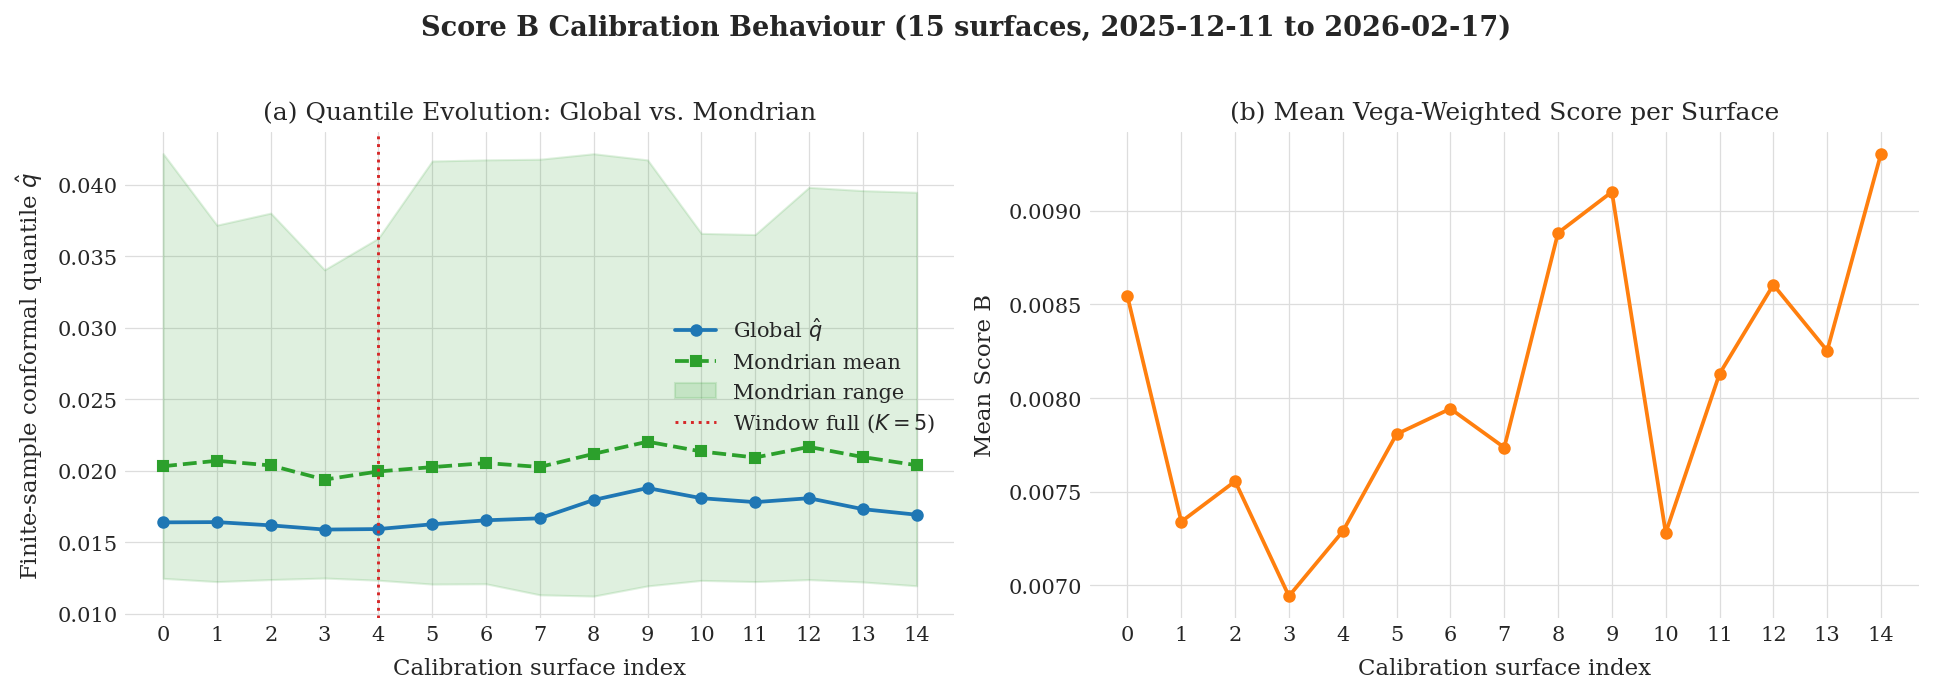
\includegraphics[width=\textwidth]{Figures/fig_quantile_evolution.png}
    \caption{Score B global quantile $\hat{q}$, Mondrian quantile range, and per-surface mean score across the 15 calibration surfaces.}
    \label{fig:quantile_evolution}
\end{figure}

\section{No-Arbitrage Projection}
\label{sec:exp_arbitrage}

The conformal construction is complemented by a post-processing step that improves the financial consistency of the lower and upper band surfaces. As discussed in Section~\ref{subsec:projection_algorithm}, the routine operates on a rectangular $(\rho,z)$ grid. The fixed-$k$ calendar condition compares consecutive maturities at the same log-moneyness $k=\rho z$. The discrete butterfly condition compares each middle total-variance value with the linearly interpolated value between its two neighbouring $z$ points. Both band surfaces are adjusted jointly so that their lower/upper ordering is included directly. The projection is applied before the final coverage and violation counts are evaluated.

\subsection{Aggregate Violation Counts}
\label{subsec:exp_arb_counts}

For each evaluation surface, fixed-$k$ calendar and discrete butterfly violations are counted separately on the lower and upper Mondrian bands and then summed. Table~\ref{tab:arbitrage} reports the aggregate counts over all 31 walk-forward evaluation surfaces. It also reports quote-level band crossings after projection, defined as locations where the projected lower bound exceeds the projected upper bound.

\begin{table}[H]
\centering
\begin{tabular}{|l|r|r|r|r|}
\hline
\textbf{Score} & \textbf{Before} & \textbf{After} & \textbf{Reduction} & \textbf{Crossings after} \\
\hline
Score A (spread) & 63{,}177 & 0 & 100.0\% & 0 \\
Score B (Vega)   & 57{,}847 & 0 & 100.0\% & 0 \\
\hline
\end{tabular}
\caption{Combined fixed-$k$ calendar and discrete butterfly violation counts on the lower and upper Mondrian bands across 31 walk-forward evaluation surfaces.}
\label{tab:arbitrage}
\end{table}

Figures~\ref{fig:calendar_arbitrage} and~\ref{fig:butterfly_arbitrage} illustrate the enforced conditions on the lower Score B band for the first evaluation surface (surface 15, 3 March 2026). The left panels show selected slices before projection and the right panels show the corresponding slices after projection. Because the figures display selected lower-band slices, their violation counts differ from the aggregate totals in Table~\ref{tab:arbitrage}.

\begin{figure}[H]
    \centering
    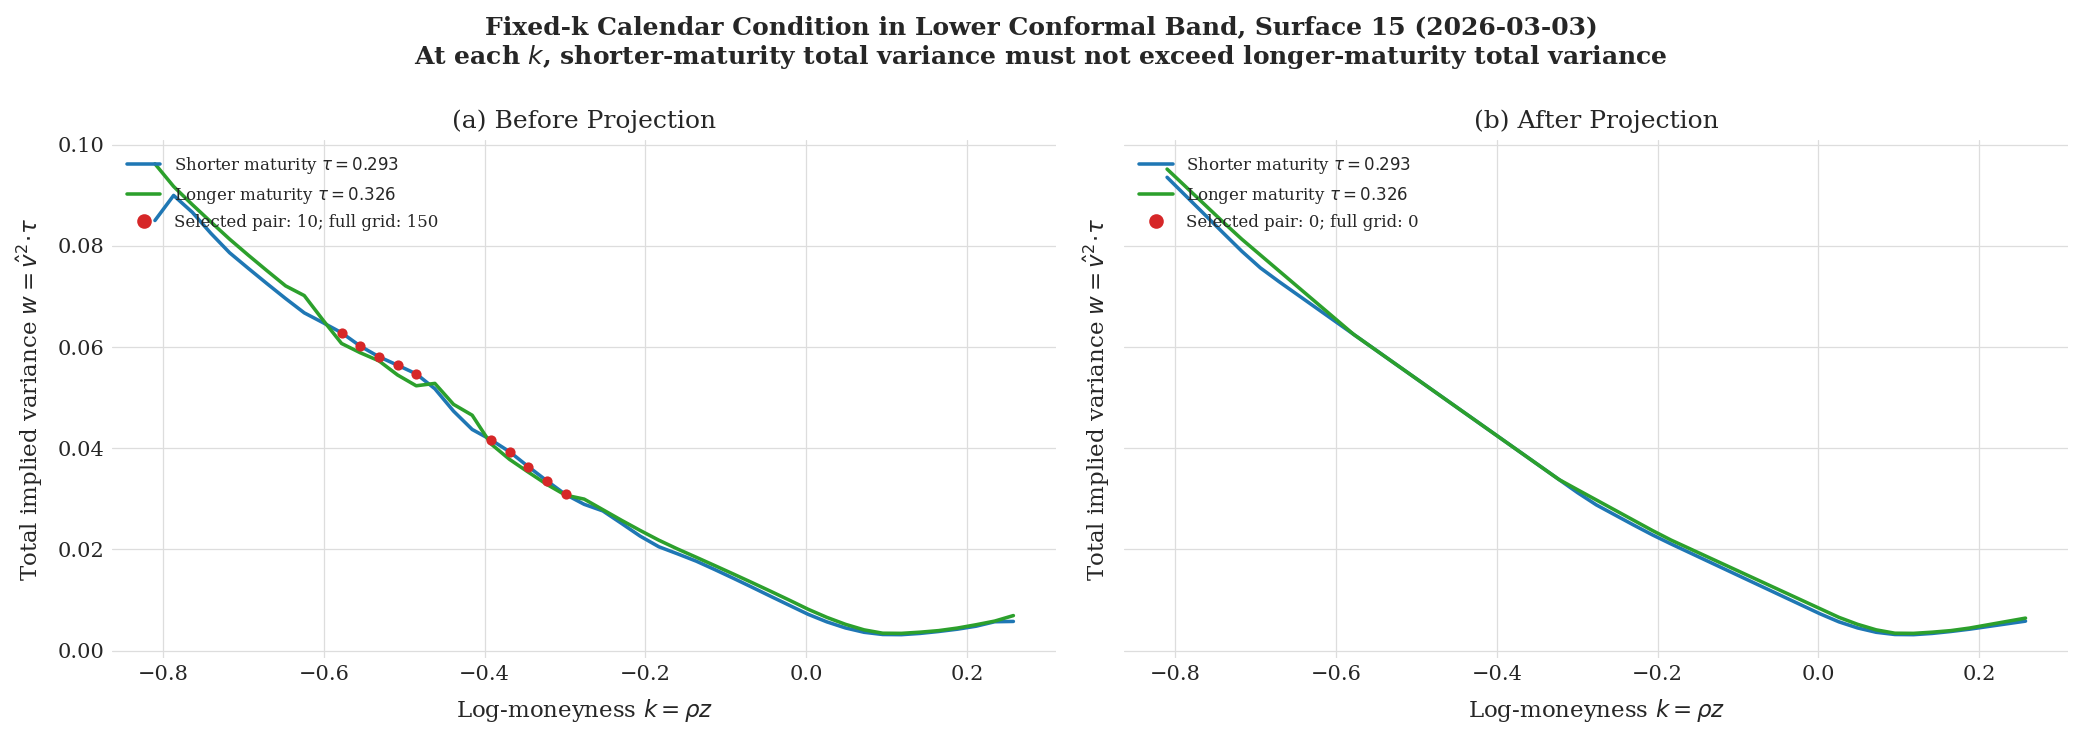
\includegraphics[width=\textwidth]{Figures/fig_calendar_arbitrage.png}
    \caption{Calendar condition in selected slices of the lower Score B band for surface 15, before and after projection.}
    \label{fig:calendar_arbitrage}
\end{figure}

\begin{figure}[H]
    \centering
    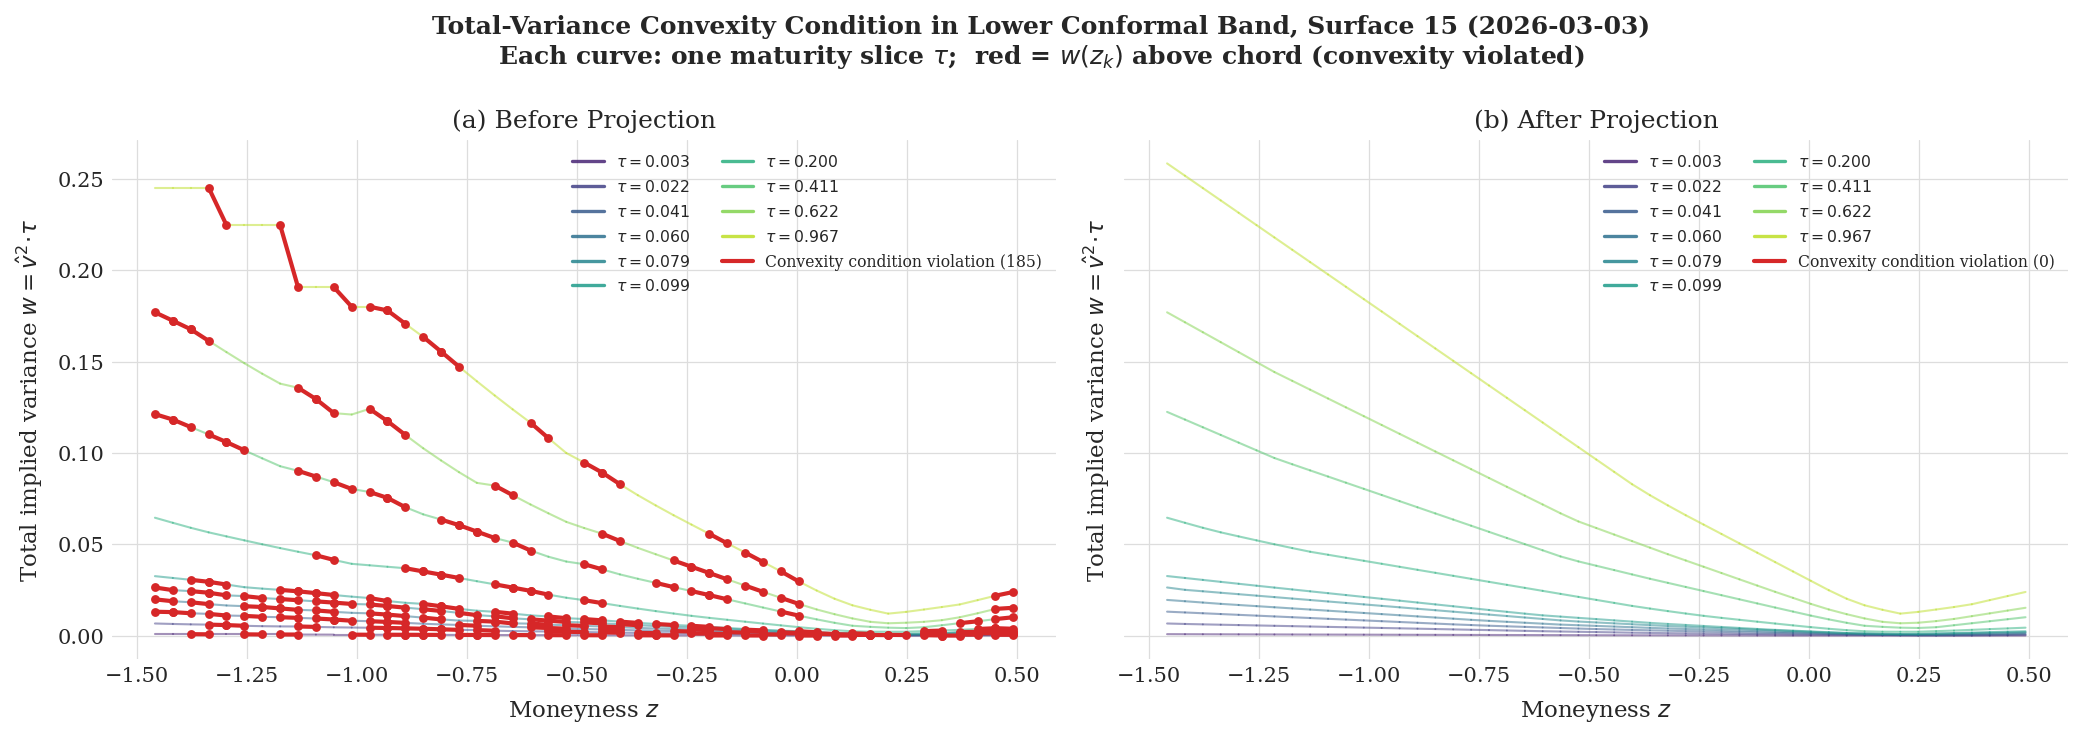
\includegraphics[width=\textwidth]{Figures/fig_butterfly_arbitrage.png}
    \caption{Discrete butterfly condition in selected maturity slices of the lower Score B band for surface 15, before and after projection.}
    \label{fig:butterfly_arbitrage}
\end{figure}

\subsection{Score B: Enforced Violations Eliminated}
\label{subsec:exp_arb_scoreb}

For Score B, the projection reaches zero residual violations of the two enforced grid conditions on every evaluation surface, reducing the combined lower-and-upper count from 57{,}847 to zero. The projected bands also have zero quote-level crossings across all 31 surfaces. This confirms that the joint linear program consistently enforces its fixed-$k$ calendar, discrete butterfly, and lower--upper ordering constraints on the discretised surfaces.

\subsection{Score A: Enforced Violations Eliminated}
\label{subsec:exp_arb_scorea}

For Score A, the same enforced violation count decreases from 63{,}177 to zero, and the projected bands have zero quote-level crossings across all 31 surfaces. The projection records 278 small positive-variance floor adjustments across both bounds for Score A, compared with none for Score B. Projection feasibility under the enforced conditions therefore does not by itself distinguish the two scores; their empirical coverage, sharpness, and numerical behaviour are compared in Section~\ref{sec:exp_ablation}.

The supplementary GNO-style butterfly diagnostic is evaluated separately and is not imposed as a constraint by the linear program. Its aggregate violation count decreases from 25{,}946 to 7{,}432 for Score A and from 27{,}906 to 2{,}731 for Score B. These non-zero diagnostic counts mean that eliminating the enforced discrete violations should not be interpreted as establishing full absence of static arbitrage under every analytic condition.

\section{Nonconformity Score Comparison}
\label{sec:exp_ablation}

The projection results in Section~\ref{sec:exp_arbitrage} show that both scores reach zero residual violations of the enforced grid conditions. The two constructions nevertheless differ materially in their band width, empirical coverage after projection, and numerical behaviour. This section compares these outcomes to explain why Score B is selected as the primary construction.

\subsection{Score Magnitude and Quantile Scale}
\label{subsec:ablation_magnitude}

The two scores use different normalisations and therefore operate at different numerical scales. Score B is a Vega-weighted IV residual. Because both experiments use the same GNO predictions, their mean prediction error is identical at MAE $=0.006813$ IV units. For Score B, the global calibration quantile is 0.016937 on the final calibration surface.

Score A is a spread-normalised price residual. On the first calibration surface (11 December 2025), its median is 1.1370, its 90th percentile is 4.0384, and its maximum is 23.3982. The corresponding global conformal quantile is 4.059961 and rises to values of approximately 20--23 as the rolling window advances, ending at 22.397682 on the final calibration surface. Score A divides the price residual by the bid--ask spread, subject to the implemented minimum spread of 0.10. Because the Score A and Score B quantiles enter different band-construction formulas, Equations~\ref{eq:price_band_halfwidth} and~\ref{eq:iv_band_halfwidth}, their raw magnitudes are not directly comparable. Their practical effects are instead compared below using IV-space band width and coverage.

\subsection{Score A Inversion and Clipping Diagnostics}
\label{subsec:score_a_diagnostics}

Score A first constructs price-space endpoints and then converts each endpoint to implied volatility. Table~\ref{tab:score_a_inversion} reports the aggregate inversion diagnostics for the 65{,}791 held-out target quotes across the 31 evaluation surfaces. Of the lower price endpoints, 58{,}190 (88.45\%) were inverted without adjustment. The remaining 7{,}601 lower endpoints (11.55\%) were negative and were therefore clipped to the minimum IV of $10^{-4}$. All upper endpoints were inverted successfully. There were no maximum-IV clips, numerical solver failures, or non-finite price endpoints for either bound.

\begin{table}[H]
\centering
\small
\begin{tabular}{|l|r|r|}
\hline
\textbf{Diagnostic} & \textbf{Lower endpoint} & \textbf{Upper endpoint} \\
\hline
Total inversions              & 65{,}791          & 65{,}791          \\
Successful inversions         & 58{,}190 (88.45\%) & 65{,}791 (100.00\%) \\
Clipped to minimum IV         & 7{,}601 (11.55\%)  & 0 (0.00\%)          \\
Clipped to maximum IV         & 0 (0.00\%)         & 0 (0.00\%)          \\
Solver failures               & 0 (0.00\%)         & 0 (0.00\%)          \\
Negative price endpoints      & 7{,}601 (11.55\%)  & 0 (0.00\%)          \\
Non-finite price endpoints    & 0 (0.00\%)         & 0 (0.00\%)          \\
\hline
\end{tabular}
\caption{Aggregate Score A price-to-IV inversion diagnostics across the 31 evaluation surfaces.}
\label{tab:score_a_inversion}
\end{table}

The minimum bid--ask spread of 0.10 was applied to 1{,}667 of the 65{,}791 target quotes (2.53\%). The diagnostics show that the numerical issue is concentrated in the lower price endpoint: more than one in ten lower endpoints fall below zero before inversion, while the upper endpoints require no clipping. This asymmetry is relevant when interpreting the post-projection coverage and width of Score A.

\subsection{Band Width}
\label{subsec:ablation_width}

Table~\ref{tab:ablation_width} reports IV band-width summaries for both scores across the 31 evaluation surfaces. Each entry gives equal weight to each surface. The post-projection median row is the mean of the 31 within-surface median widths.

\begin{table}[H]
\centering
\begin{tabular}{|l|c|c|}
\hline
\textbf{Metric} & \textbf{Score A (spread)} & \textbf{Score B (vega)} \\
\hline
Mean width before projection (IV)       & 0.060798 & 0.027111 \\
Mean width after projection (IV)        & 0.067806 & 0.027180 \\
Mean post-projection median width (IV)  & 0.033759 & 0.025862 \\
Mean width change from projection       & 9.88\%   & 0.26\%   \\
\hline
\end{tabular}
\caption{Surface-weighted IV band-width summaries across the 31 evaluation surfaces.}
\label{tab:ablation_width}
\end{table}

After projection, Score A is approximately 2.5 times wider than Score B in mean IV width and 1.3 times wider in the mean of the per-surface median widths. Projection increases the mean Score A width by 9.88\%, whereas the mean Score B width changes by only 0.26\%. Score B therefore provides sharper bands and is substantially less sensitive to the projection step.

\subsection{Coverage Across Evaluation Surfaces}
\label{subsec:ablation_coverage}

Table~\ref{tab:ablation_coverage} reports the post-projection per-surface Mondrian coverage for both scores alongside the overall mean and standard deviation across all 31 evaluation surfaces. The summary statistics give equal weight to each surface; they are not calculated by pooling all quotes across dates.

\begin{table}[H]
\centering
\small
\begin{tabular}{|c|l|c|c|}
\hline
\textbf{Idx} & \textbf{Date} & \textbf{Score A coverage} & \textbf{Score B coverage} \\
\hline
15 & 2026-03-03 & 91.31\% & 91.42\% \\
16 & 2026-04-10 & 73.81\% & 91.60\% \\
17 & 2026-04-16 & 82.98\% & 94.36\% \\
18 & 2026-04-17 & 79.36\% & 89.39\% \\
19 & 2026-05-08 & 82.05\% & 96.37\% \\
20 & 2026-05-13 & 82.16\% & 91.20\% \\
21 & 2026-05-14 & 86.38\% & 95.58\% \\
22 & 2026-05-15 & 83.71\% & 94.45\% \\
23 & 2026-05-18 & 80.06\% & 94.53\% \\
24 & 2026-05-19 & 92.32\% & 91.91\% \\
25 & 2026-05-20 & 92.39\% & 94.47\% \\
26 & 2026-05-21 & 96.17\% & 94.93\% \\
27 & 2026-05-22 & 85.13\% & 94.77\% \\
28 & 2026-06-04 & 82.18\% & 89.37\% \\
29 & 2026-06-05 & 72.13\% & 91.36\% \\
30 & 2026-06-16 & 81.77\% & 93.51\% \\
31 & 2026-06-23 & 85.17\% & 93.36\% \\
32 & 2026-06-24 & 94.29\% & 93.60\% \\
33 & 2026-06-26 & 84.83\% & 94.02\% \\
34 & 2026-07-02 & 87.74\% & 93.14\% \\
35 & 2026-07-07 & 82.02\% & 91.25\% \\
36 & 2026-07-08 & 76.25\% & 92.24\% \\
37 & 2026-07-15 & 85.53\% & 95.40\% \\
38 & 2026-07-17 & 86.28\% & 95.83\% \\
39 & 2026-07-30 & 94.67\% & 91.04\% \\
40 & 2026-07-31 & 81.43\% & 92.07\% \\
41 & 2026-08-04 & 86.88\% & 93.01\% \\
42 & 2026-08-05 & 89.88\% & 88.93\% \\
43 & 2026-08-06 & 77.72\% & 91.00\% \\
44 & 2026-08-07 & 72.80\% & 91.98\% \\
45 & 2026-08-11 & 82.81\% & 92.33\% \\
\hline
\textbf{Mean} & & \textbf{84.27\%} & \textbf{92.85\%} \\
\textbf{Std}  & & \textbf{6.24\%}  & \textbf{1.97\%}  \\
\hline
\end{tabular}
\caption{Post-projection per-surface Mondrian coverage for Score A and Score B across all 31 evaluation surfaces. Target: $1-\alpha=90\%$.}
\label{tab:ablation_coverage}
\end{table}

Figure~\ref{fig:coverage_comparison} shows the post-projection per-surface coverage for both scores, together with the 90\% nominal target. Figure~\ref{fig:band_width_comparison} separately shows their mean IV band widths across the same 31 evaluation surfaces.

\begin{figure}[H]
    \centering
    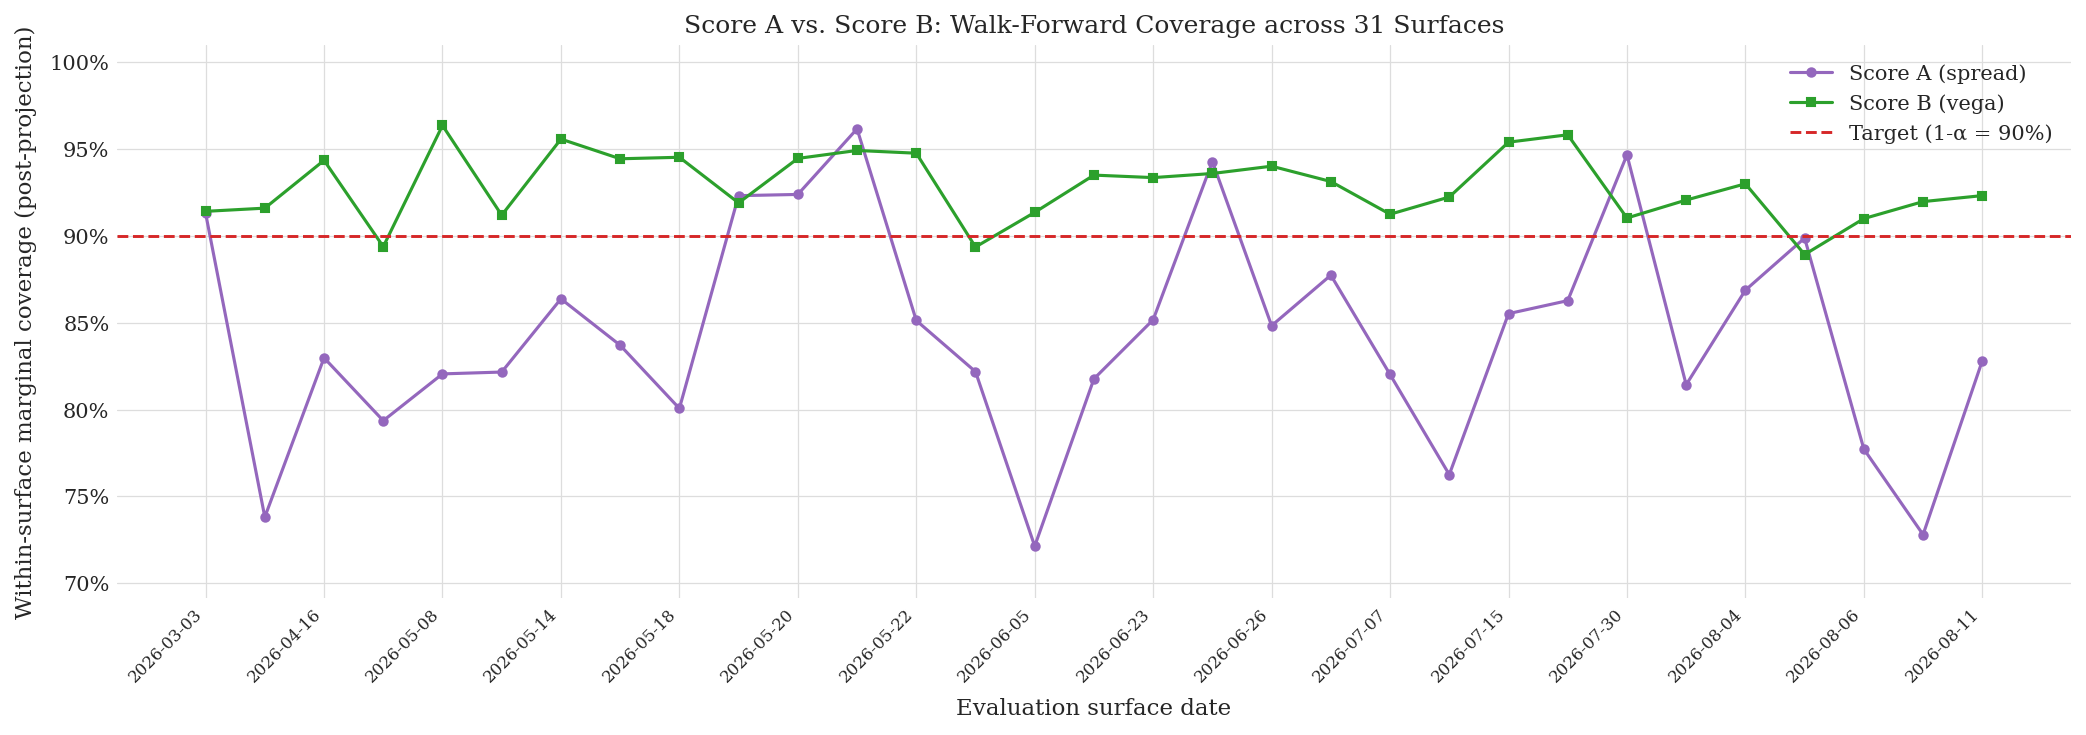
\includegraphics[width=\textwidth]{Figures/fig_coverage_comparison.png}
    \caption{Post-projection per-surface Mondrian coverage for Score A and Score B across the 31 evaluation surfaces.}
    \label{fig:coverage_comparison}
\end{figure}

\begin{figure}[H]
    \centering
    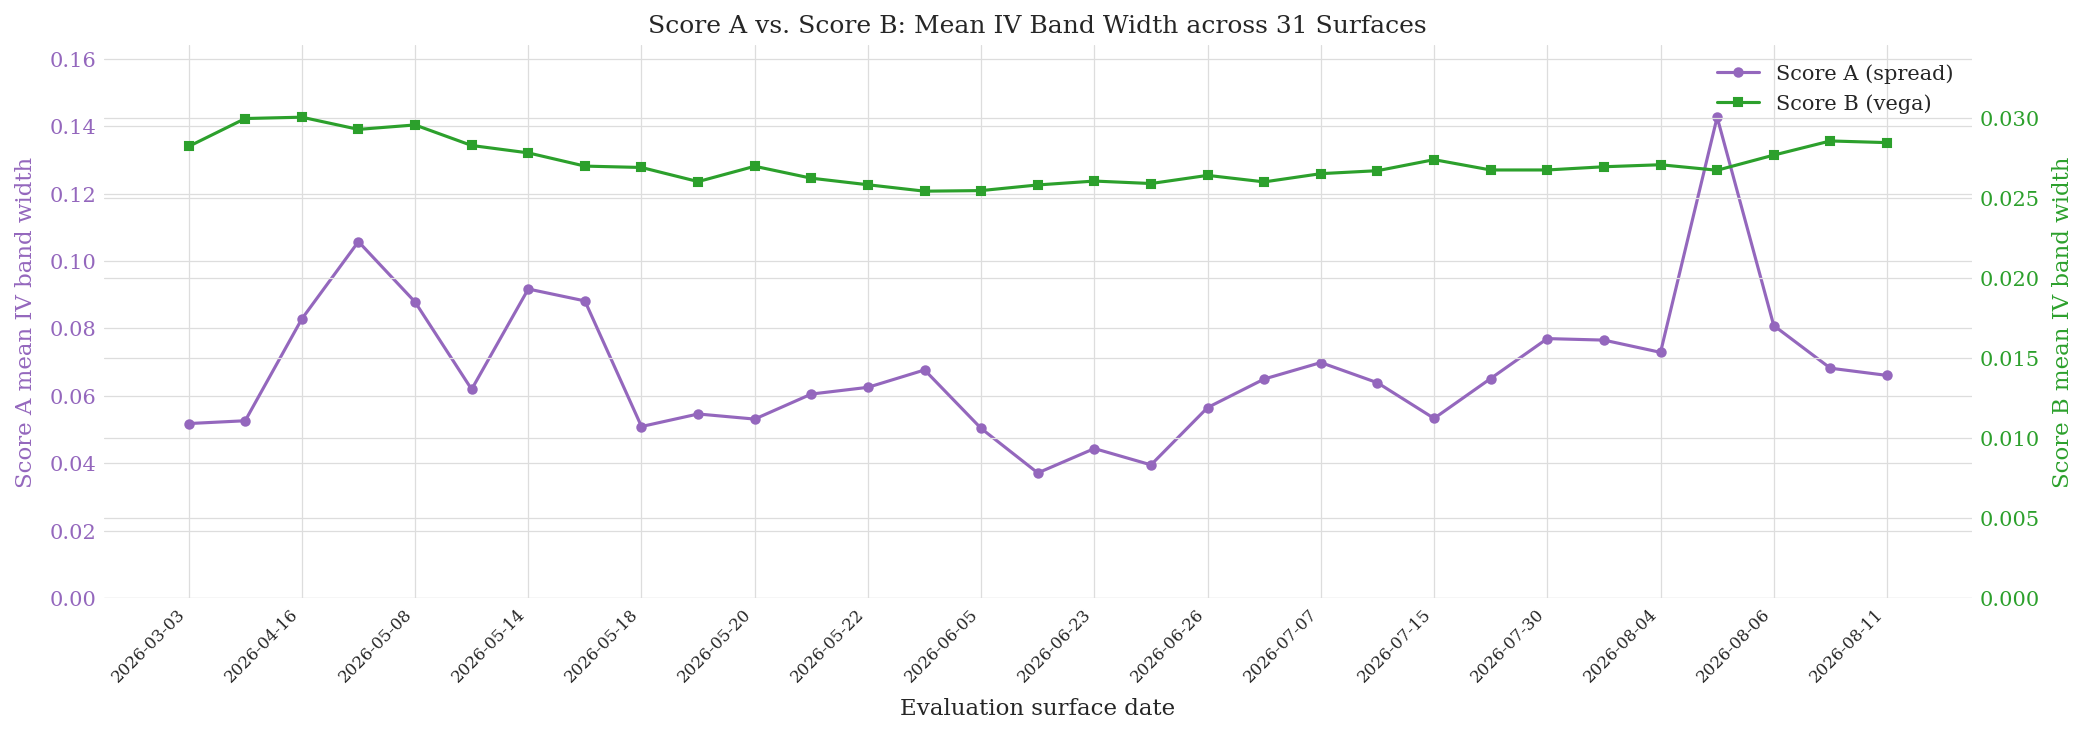
\includegraphics[width=\textwidth]{Figures/fig_band_width_comparison.png}
    \caption{Post-projection mean IV band width for Score A and Score B across the 31 evaluation surfaces. The two vertical axes show the different width scales of the two scores.}
    \label{fig:band_width_comparison}
\end{figure}

Before projection, mean Mondrian coverage is 90.19\% for Score A and 91.11\% for Score B. After projection, Score A coverage decreases to 84.27\%, whereas Score B coverage increases to 92.85\%. The surface-bootstrap 95\% confidence interval for the post-projection mean is $[82.10\%,86.42\%]$ for Score A and $[92.19\%,93.52\%]$ for Score B.

Post-projection Score A coverage ranges from 72.13\% to 96.17\% and falls below the nominal target on 25 of the 31 surfaces. Its standard deviation is 6.24 percentage points. Score B ranges from 88.93\% to 96.37\%, falls below the target on three surfaces, and has a standard deviation of 1.97 percentage points. Score B therefore provides both higher mean coverage and substantially greater temporal stability after projection.

\subsection{Summary of Score Comparison}
\label{subsec:ablation_summary}

Both scores reach zero violations of the enforced calendar and discrete butterfly conditions, so that result alone does not determine the preferred construction. Score A begins near the nominal coverage level before projection but loses coverage and becomes wider after the projection step. Score B remains narrow, changes little in width, and achieves a post-projection mean coverage of 92.85\% with lower variation across surfaces. These outcomes reflect the direct IV construction of Score B versus the price-to-IV inversion of Score A. Accordingly, Sections~\ref{sec:exp_coverage} and~\ref{sec:exp_sharpness} report Score B as the recommended construction.

\section{Coverage Results}
\label{sec:exp_coverage}

This section examines the empirical marginal coverage of the Score B framework in detail across the 31 held-out evaluation surfaces. Coverage is the fraction of market implied volatility quotes that fall within the constructed band at each evaluation surface, as defined in Section~\ref{sec:meth_metrics}. Two variants are reported at the same post-projection stage: the global construction uses a single scalar quantile from the rolling window, whereas the Mondrian construction uses per-bin quantiles from the same window. Both use the same $L=5$ rolling window and the same projection routine; the difference is the quantile assignment.

\subsection{Per-Surface Coverage}
\label{subsec:exp_coverage_persurface}

Table~\ref{tab:coverage_scoreb} reports the matched post-projection global and Mondrian coverage for Score B on each evaluation surface. The mean and standard deviation give equal weight to each of the 31 surface-level coverage values.

\begin{table}[H]
\centering
\small
\begin{tabular}{|c|l|c|c||c|l|c|c|}
\hline
\textbf{Idx} & \textbf{Date} & \textbf{Global} & \textbf{Mondrian} &
\textbf{Idx} & \textbf{Date} & \textbf{Global} & \textbf{Mondrian} \\
\hline
15 & 2026-03-03 & 88.12\% & 91.42\% & 31 & 2026-06-23 & 90.41\% & 93.36\% \\
16 & 2026-04-10 & 91.13\% & 91.60\% & 32 & 2026-06-24 & 90.05\% & 93.60\% \\
17 & 2026-04-16 & 91.20\% & 94.36\% & 33 & 2026-06-26 & 90.18\% & 94.02\% \\
18 & 2026-04-17 & 89.30\% & 89.39\% & 34 & 2026-07-02 & 90.72\% & 93.14\% \\
19 & 2026-05-08 & 93.72\% & 96.37\% & 35 & 2026-07-07 & 88.01\% & 91.25\% \\
20 & 2026-05-13 & 89.52\% & 91.20\% & 36 & 2026-07-08 & 89.26\% & 92.24\% \\
21 & 2026-05-14 & 92.73\% & 95.58\% & 37 & 2026-07-15 & 93.59\% & 95.40\% \\
22 & 2026-05-15 & 92.03\% & 94.45\% & 38 & 2026-07-17 & 94.57\% & 95.83\% \\
23 & 2026-05-18 & 92.60\% & 94.53\% & 39 & 2026-07-30 & 90.14\% & 91.04\% \\
24 & 2026-05-19 & 89.59\% & 91.91\% & 40 & 2026-07-31 & 91.44\% & 92.07\% \\
25 & 2026-05-20 & 90.87\% & 94.47\% & 41 & 2026-08-04 & 89.19\% & 93.01\% \\
26 & 2026-05-21 & 90.50\% & 94.93\% & 42 & 2026-08-05 & 88.84\% & 88.93\% \\
27 & 2026-05-22 & 93.25\% & 94.77\% & 43 & 2026-08-06 & 90.25\% & 91.00\% \\
28 & 2026-06-04 & 90.11\% & 89.37\% & 44 & 2026-08-07 & 92.25\% & 91.98\% \\
29 & 2026-06-05 & 89.64\% & 91.36\% & 45 & 2026-08-11 & 89.52\% & 92.33\% \\
30 & 2026-06-16 & 92.02\% & 93.51\% & & & & \\
\hline
\multicolumn{2}{|c|}{\textbf{Mean}} & \textbf{90.80\%} & \textbf{92.85\%} & & & & \\
\multicolumn{2}{|c|}{\textbf{Std}} & \textbf{1.67\%} & \textbf{1.97\%} & & & & \\
\hline
\end{tabular}
\caption{Matched post-projection Score B coverage on all 31 evaluation surfaces ($1-\alpha=90\%$).}
\label{tab:coverage_scoreb}
\end{table}

Over the full 31-surface evaluation period, the mean Mondrian coverage is 92.85\%, above the 90\% nominal target. Its standard deviation is 1.97 percentage points, and the surface-bootstrap 95\% confidence interval for its mean is $[92.19\%,93.52\%]$. The minimum Mondrian coverage is 88.93\% (surface 42, 5 August 2026), and the maximum is 96.37\% (surface 19, 8 May 2026). Mondrian coverage falls below the 90\% target on three evaluation surfaces.

\subsection{Contribution of Mondrian Spatial Binning}
\label{subsec:exp_mondrian_contribution}

The global coverage column of Table~\ref{tab:coverage_scoreb} provides the comparison without spatial binning while retaining the same rolling window and projection stage. Its mean coverage is 90.80\%, compared with 92.85\% for Mondrian coverage.

Mondrian spatial binning raises mean post-projection coverage by 2.05 percentage points. For example, coverage increases from 88.12\% to 91.42\% on surface 15 and from 89.19\% to 93.01\% on surface 41. Across the evaluation period, eight surfaces have global coverage below 90\% but Mondrian coverage at or above 90\%. These results indicate that assigning calibration quantiles by surface region reduces undercoverage on several evaluation dates. The cross-surface standard deviation is 1.67 percentage points for global coverage and 1.97 percentage points for Mondrian coverage, so the improvement in mean coverage is not accompanied by lower temporal variation.

The three surfaces where Mondrian coverage remains below 90\% are surfaces 18, 28, and 42. Global coverage reaches at least 90\% only on surface 28, showing that Mondrian binning improves average coverage but does not increase coverage on every individual surface. At each walk-forward step, coverage is evaluated using the preceding rolling window; the current surface is added only after its evaluation and can then contribute to the next window. The window therefore contains the five most recently processed surfaces without using future information. The remaining temporal variation and its relation to the conformal assumptions are discussed further in Chapter~\ref{chap:discussion}.

Figure~\ref{fig:spatial_coverage_comparison} compares post-projection global and Mondrian coverage within each cell of the $4\times4$ partition. Coverage is first calculated within each populated bin on every evaluation surface and then averaged across surfaces, so that dates with more target quotes do not receive greater weight.

\begin{figure}[H]
    \centering
    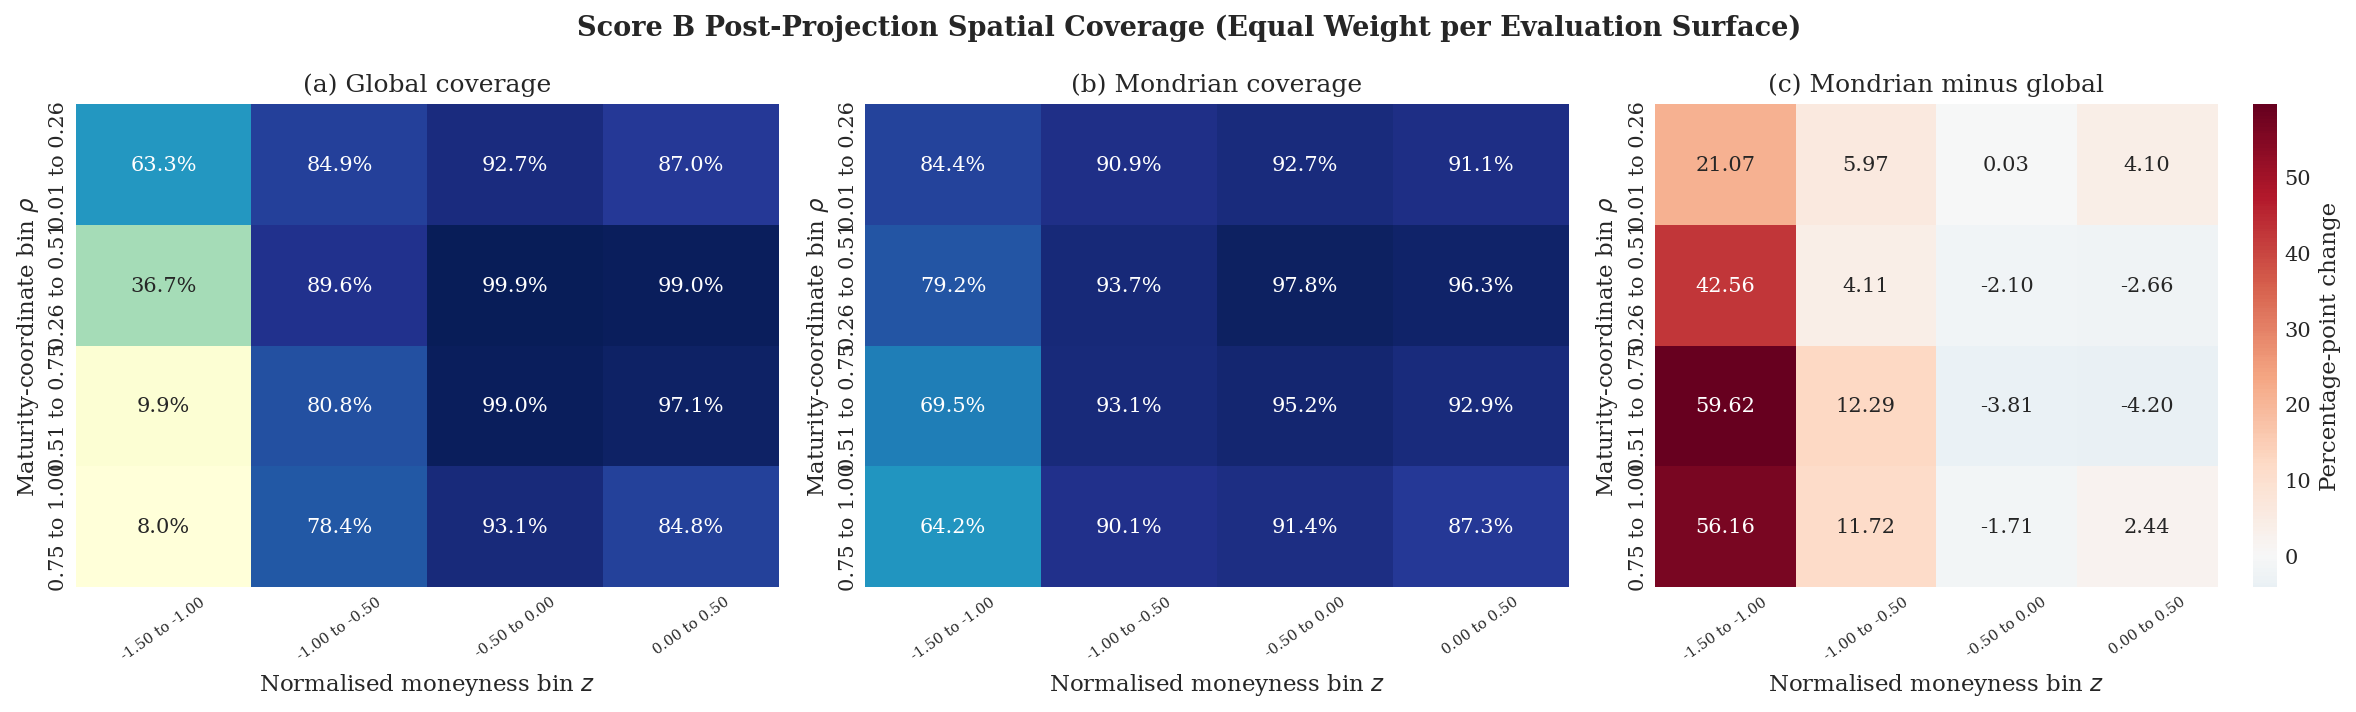
\includegraphics[width=\textwidth]{Figures/fig_spatial_coverage_comparison.png}
    \caption{Surface-weighted post-projection Score B coverage by $(\rho,z)$ bin for global and Mondrian calibration. The right panel reports the Mondrian-minus-global change in percentage points.}
    \label{fig:spatial_coverage_comparison}
\end{figure}

The largest increases occur in the lowest-moneyness column, $z\in[-1.5,-1.0]$, where the change ranges from 21.07 to 59.62 percentage points across the four maturity bins. Despite these increases, Mondrian coverage in this column remains between 64.2\% and 84.4\%, below the nominal target in every maturity bin. In the remaining cells, changes range from $-4.20$ to 12.29 percentage points. Mondrian calibration therefore reduces severe spatial undercoverage in the lowest-moneyness region, but it does not eliminate it and does not improve coverage in every bin.

\section{Sharpness}
\label{sec:exp_sharpness}

Sharpness is assessed through the width of the prediction bands at the held-out target quotes. Coverage alone does not distinguish a narrow band from an unnecessarily wide one, so band width is reported alongside coverage. The results below concern the post-projection Mondrian bands on the 31 evaluation surfaces.

\subsection{Overall Band Width}
\label{subsec:exp_width_overall}

Averaging the per-surface mean IV band widths across the 31 evaluation surfaces, with equal weight given to each surface, gives 0.027180 IV units. The surface-bootstrap 95\% confidence interval for this mean is $[0.026755,0.027636]$. The corresponding equal-weight average of the per-surface median widths is 0.025862 IV units. These values are computed at the scattered target quotes after the projected grid values have been mapped back to the original $(\rho,z)$ coordinates.

Before projection, the mean Score B width is 0.027111 IV units. Projection raises it by 0.000069 IV units on average, corresponding to an increase of 0.255\%. The GNO point-prediction MAE is 0.006813 IV units. The post-projection mean half-width of 0.013590 IV units is therefore approximately twice the MAE. Together with the mean Mondrian coverage of 92.85\%, these values summarise the observed coverage and band width of Score B.

\subsection{Spatial Variation of Band Width}
\label{subsec:exp_width_spatial}

The Mondrian construction permits spatially varying band widths by assigning calibration quantiles according to the $(\rho,z)$ bin containing each point. On surface 14, the last surface in the initial calibration period, the bin quantiles range from $0.011970$ to $0.039470$ (Table~\ref{tab:calibration_quantiles}). The largest threshold is approximately 3.3 times the smallest. This comparison concerns the calibration thresholds, not the final band widths, which also depend on the local Vega weight and the projection. As shown in Section~\ref{subsec:exp_mondrian_contribution}, the spatial assignment increases mean post-projection coverage relative to the global construction, although it does not increase coverage on every surface.

Figure~\ref{fig:uncertainty_surface} illustrates the post-projection Score B bands for the first evaluation surface, dated 3 March 2026. The left panel shows the GNO estimate together with the lower and upper conformal surfaces. The right panel shows the pointwise distance between the two conformal surfaces in IV units.

\begin{figure}[H]
    \centering
    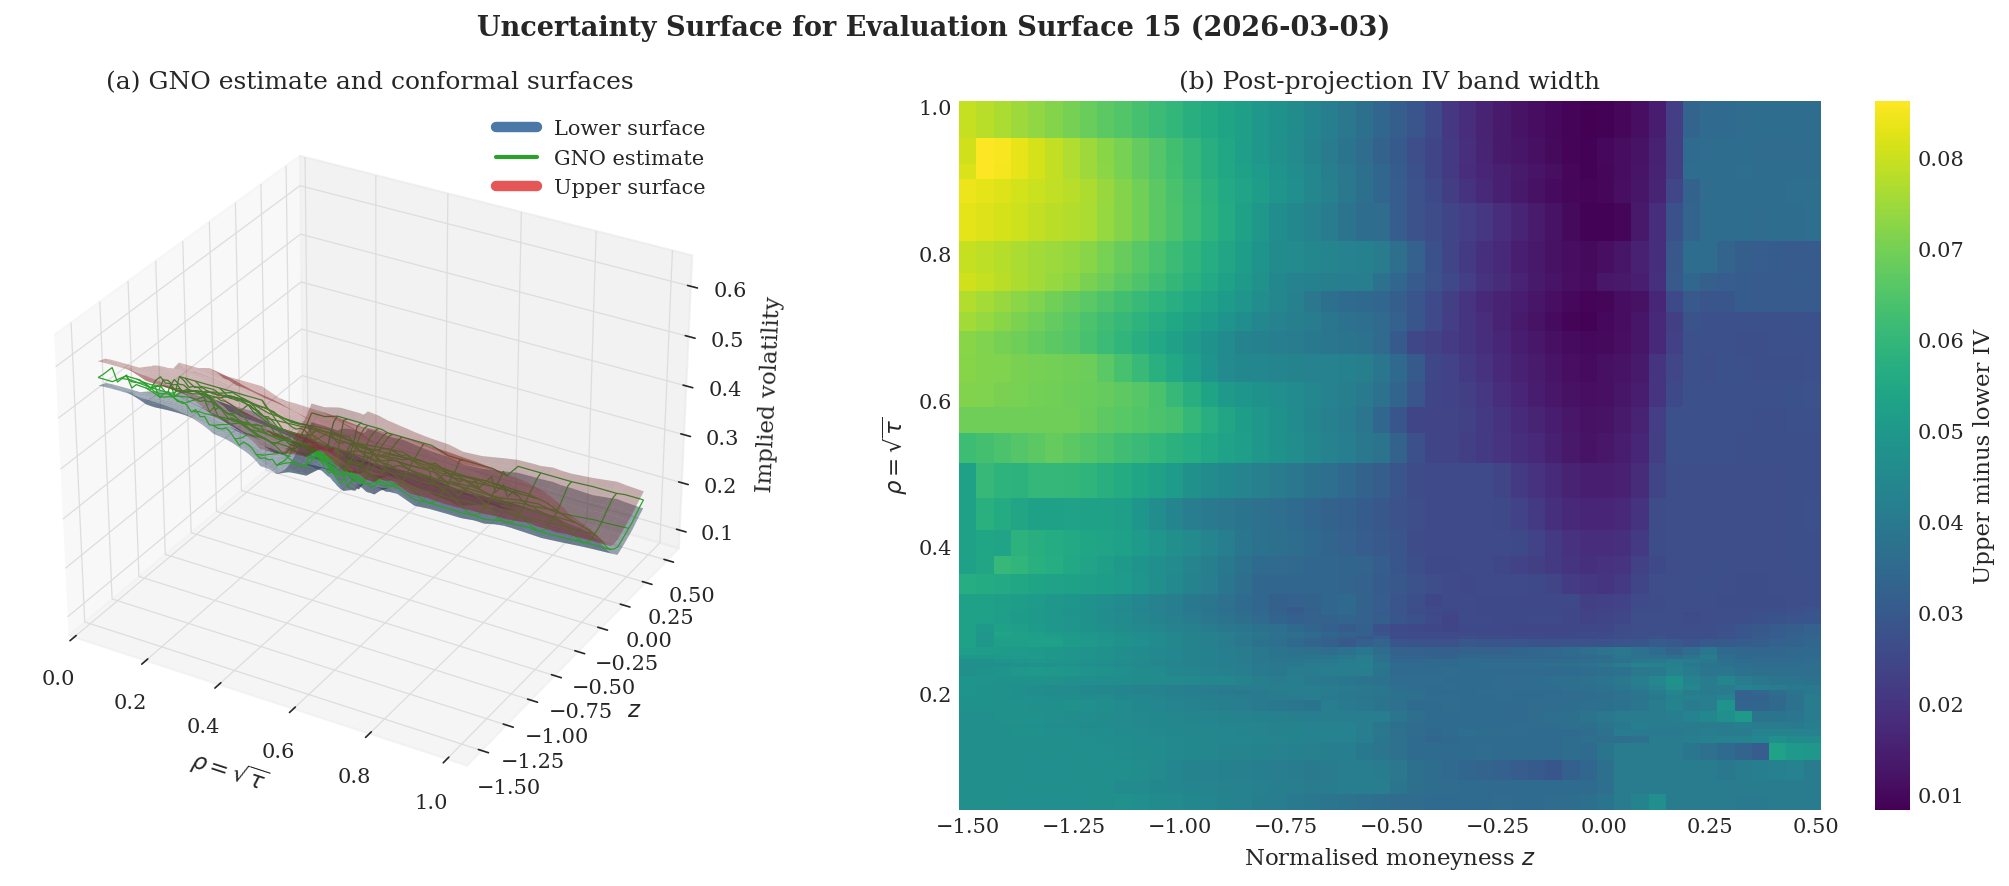
\includegraphics[width=\textwidth]{Figures/fig_uncertainty_surface.png}
    \caption{GNO implied-volatility estimate, post-projection lower and upper Score B conformal surfaces, and the corresponding IV band width for evaluation surface 15.}
    \label{fig:uncertainty_surface}
\end{figure}

For this surface, the largest widths occur mainly at negative normalised moneyness and longer maturities. The smallest widths appear near the centre of the moneyness range at longer maturities. This figure provides one spatial example; the aggregate width and coverage results use all 31 evaluation surfaces.

\subsection{Sharpness Relative to Score A}
\label{subsec:exp_width_vs_scorea}

The comparison in Section~\ref{subsec:ablation_width} uses the same 31 evaluation surfaces and the same post-projection stage for both scores. Score A has a mean band width of 0.067806 IV units, approximately 2.49 times the Score B mean of 0.027180. Its mean Mondrian coverage is 84.27\%, compared with 92.85\% for Score B. In this experiment, Score B therefore has both the narrower mean band and the higher post-projection coverage. The difference reflects the score constructions: Score A calibrates spread-normalised price residuals and maps price bands into IV space, whereas Score B forms the bands from Vega-weighted IV residuals.

\clearpage
\section{Summary}
\label{sec:exp_summary}

The evaluation began with 56 collected S\&P 500 option surface files. After excluding ten files whose collection dates did not correspond to regular trading sessions, 46 surfaces remained. The first 15 formed the initial calibration period, and the remaining 31 were processed in walk-forward order with a rolling window of size $L=5$.

During the initial calibration period, the Score B global quantile ranged from 0.015899 to 0.018801. On surface 14, the final surface in this period, the Mondrian bin quantiles ranged from 0.011970 to 0.039470. The largest bin threshold was therefore approximately 3.3 times the smallest, reflecting spatial differences in the calibrated scores.

Across the 31 evaluation surfaces, Score B achieved mean post-projection Mondrian coverage of 92.85\%, with a surface-bootstrap 95\% confidence interval of $[92.19\%,93.52\%]$. The corresponding global coverage was 90.80\%. Mondrian coverage was below the 90\% target on three surfaces. The mean post-projection Score B width was 0.027180 IV units, with a 95\% confidence interval of $[0.026755,0.027636]$, while the GNO point-prediction MAE was 0.006813 IV units. Projection increased the mean Score B width by 0.255\%.

The joint projection eliminated all violations of the enforced calendar and discrete butterfly conditions for both scores. The combined count fell from 63{,}177 to zero for Score A and from 57{,}847 to zero for Score B, with no lower and upper band crossings at the target quotes. The supplementary GNO-style butterfly diagnostic was not imposed as a constraint and remained nonzero after projection: its aggregate count decreased from 25{,}946 to 7{,}432 for Score A and from 27{,}906 to 2{,}731 for Score B.

The comparison of the two scores used the same predictions and evaluation surfaces. Score A had mean post-projection Mondrian coverage of 84.27\%, a coverage standard deviation of 6.24 percentage points, and a mean width of 0.067806 IV units. For Score B, the corresponding values were 92.85\%, 1.97 percentage points, and 0.027180 IV units. Score A was approximately 2.49 times wider on average while having lower coverage. Score B is therefore retained as the primary construction for the discussion in Chapter~\ref{chap:discussion}, where the temporal variation in coverage, the conformal assumptions, and the limitations of the projection diagnostics are examined.
